\documentclass[report.tex]{subfiles}

\begin{document}

\chapter{Background material}

This chapter provides the material necessary for understanding the
Bouncy Particle Sampler (BPS) algorithm which relies on simulation of a
piecewise-deterministic Markov process.
We introduce the material necessary
for understanding the simulation and analysis of such processes.
This chapter is complemented by Appendix~\ref{appendix-metropolis-hastings}
where we also introduce the Metropolis-Hastings algorithm
-- a cornerstone for many MCMC algorithms including the BPS.


\section{Non-homogeneous Poisson processes simulation}
\label{background-material-poisson-processes}


Non-homogeneous Poisson processes play a central role in the simulation of
piecewise-deterministic Markov processes. We will later see that it is
the main source of randomness in the Bouncy Particle Sampler algorithm.
In this section we first give the definition of homogeneous Poisson processes
and then discuss why such processes appear so naturally in many real-world applications.
Next, we generalize to the non-homogeneous case and present a number of different
simulation techniques.
We mostly refer to textbooks by
\citet{devroye2013non},
\citet{feller1968Introduction} and
\citet{ross1996stochastic},
where more careful treatment of the following material can be found.

\subsection{Homogeneous Poisson process}

Consider a sequence of events occuring at random times
$0 < T_{1} < T_{2} < \dots$ Let $N$ be a counting process, given by
$\countingProcess{N}{s}{t} \coloneqq \# \{ i \mid T_{i} \in (s, t] \}$ where
$0 \leq s \leq t$.
In many rea-world applications, such as modelling the number of incoming
phone calls at a telephone call centre or the number of decays from a
radioactive source in a given time interval, the following assumptions are met:

\begin{enumerate}
  \item \textbf{Independent increments.} \\
  Let $0 \leq s_{1} \leq t_{1} \leq s_{2} \leq \dots \leq s_{n} \leq t_{n}$.
  Then the random variables
  \countingProcess{N}{s_{1}}{t_{1}}, \dots, \countingProcess{N}{s_{n}}{t_{n}}
  are independent.

  \item \textbf{Stationarity.} \\
  For any $0 \leq s \leq t$ the random variables
  \countingProcess{N}{s}{t} and \countingProcess{N}{0}{t-s}
  have the same distribution, so that the number of events in a given time
  interval depends only on the length of that interval.
\end{enumerate}

\noindent
The remarkable consequence of these conditions is that $\exists \lambda \geq 0$
such that for any $0 \leq s \leq t$ the random variable
\countingProcess{N}{s}{t} has a Poisson distribution with parameter $\lambda(t-s)$.

We now sketch a proof of the above claim
(see \cite{feller1968Introduction} for full details).
Assume that $\ex{\countingProcess{N}{0}{1}} = \lambda < \infty$.
Partition an interval of unit length into $m$ subintervals of length
$h \coloneqq m^{-1}$. By the two conditions above, the number of events in each
of these subintervals are independent and identically distributed (i.i.d)
with distribution of \countingProcess{N}{0}{h}.
Let $p_{k}(h)$ be a shorthand for $\pr{\countingProcess{N}{0}{h} = k}$.
Then the expected number of subintervals containing at least one event is
$h^{-1}(1 - p_{0}(h))$.
Intuitively, as $h \to 0$ the number of subintervals containing more than one
event vanishes and hence we expect that
$\lim_{h \to 0}h^{-1}(1 - p_{0}(h)) = \lambda$.
Hence we can write
\begin{equation}
\begin{split}
  \label{hom-pp-characterization}
  p_{0}(h) &= 1 - \lambda h + o(h), \\
  p_{1}(h) &= \lambda h + o(h).
\end{split}
\end{equation}
The proof concludes by considering $p_{k}(t + h)$ conditioned on the number of
events that happened up to time $t$, which allows us to derive a set of ordinary
differential equations whose solutions confirm that
$\countingProcess{N}{0}{t} \sim \text{Poisson}(\lambda t)$ for any $t \geq 0$.

Finally, note that for $k \in \mathbb{N}$ we have
$
  \cpr{T_{k+1} > T_{k} + t}{T_{k}}
  = \pr{\countingProcess{N}{0}{t} = 0}
  = \myexp{-\lambda t}
$
and hence the interarrival time $T_{k+1} - T_{k}$ conditioned on $T_{k}$
is exponentially distributed with parameter $\lambda$. From independent
increments and stationarity conditions it also follows that interarrival times
are independent. Hence, we can simulate a homogeneous Poisson process
with rate $\lambda$ using Algorithm~\ref{alg-hom-pp}.

\begin{algorithm}
\caption{Homogeneous Poisson process simulation}
\label{alg-hom-pp}
\begin{algorithmic}
  \State{$T_{0} \gets 0$}
  \For{$i = 1, 2, \dots$}
    \State{$\text{Generate } U \sim \text{Uniform}(0, 1)$}
    \State{$E_{\lambda} \gets -\frac{\log(U)}{\lambda}$}
    \Comment{$E_{\lambda}$ is an Exponential random variable with rate $\lambda$}
    \State{$T_{i} \gets T_{i-1} + E_{\lambda}$}
  \EndFor
\end{algorithmic}
\end{algorithm}

\subsection{Generalising to the non-homogeneous case}
\label{non-hom-pp-background}

Suppose we want to model the number of customers arriving at a supermarket.
While it is reasonable to assume that different customers arrive independently
of one another, the customer counting process is not stationary -- the number
of customers will clearly be larger in the evening than, for example, during
the regular working hours.
We can model such processes by dropping the stationarity condition introduced
in the previous section.

Instead of parameterizing our process by some constant $\lambda \geq 0$, we introduce
an intensity function $\lambda(t) \geq 0$, where $t$ is the time parameter, and
further assume that $\myint{0}{\infty}{\lambda(s)}{s} = \infty$.
Let $p_{k}(t, h)$ be a shorthand for $\pr{\countingProcess{N}{t}{t+h} = k}$.
The price we pay for non-stationarity is that Equations~\ref{hom-pp-characterization}
become:
\begin{equation}
\begin{split}
  \label{non-hom-pp-characterization}
  p_{0}(t, h) &= 1 - \lambda(t) h + o(h), \\
  p_{1}(t, h) &= \lambda(t) h + o(h).
\end{split}
\end{equation}
Let $\Lambda(t) \coloneqq \myint{0}{t}{\lambda(s)}{s}$ where $t \geq 0$.
Just like in the homogeneous case, by considering $p_{k}(s, t + h)$,
conditioning on the number of events that happened between times $s$ and $s + t$
and using equations given in \ref{non-hom-pp-characterization},
we can derive a set of differential equations, whose unique solution shows that
$\countingProcess{N}{s}{t+s} \sim \text{Poisson}(\Lambda(t+s) - \Lambda(s))$.
We can see that if $\lambda(t)$ is constant, then Equations~\ref{non-hom-pp-characterization}
do not depend ont $t$ and we go back to Equations~\ref{hom-pp-characterization}
for the homogeneous Poisson process.
We will now present three techniques for non-homogeneous Poisson process simulation,
all of which can be found in \citet{devroye2013non}.

\subsubsection{Simulation by time scale transformation}

A non-homogeneous Poisson process can be seen as a homogeneous Poisson process
under a certain time scale transformation.
Let $\{\countingProcess{N}{0}{t} \mid t \geq 0\}$
be a Poisson process of rate $1$ and define a new counting process
$\countingProcess{M}{0}{t} \coloneqq \countingProcess{N}{0}{\Lambda(t)}$.
Since $\Lambda(t)$ is non-decreasing, $M$ has the independent increments property.
Also $\countingProcess{M}{s}{t}$ is distributed as
$\countingProcess{N}{\Lambda(s)}{\Lambda(t)} \sim \text{Poisson}(\Lambda(t) - \Lambda(s))$
which is enough to recover Equations~\ref{non-hom-pp-characterization}.
Hence, $\{\countingProcess{M}{0}{t} \mid t \geq 0\}$ is a non-homogeneous Poisson process
with intensity function $\lambda(t)$. See Figure~\ref{image-pp-time-scale-transformation}
for a graphical representation.
Algorithm~\ref{alg-non-hom-pp-time-scale} shows how the above idea can be used to
simulate a non-homogeneous Poisson process.
\begin{algorithm}
\caption{Non-homogeneous Poisson process simulation by time scale transformation}
\label{alg-non-hom-pp-time-scale}
\begin{algorithmic}[1]
  \State{$T_{0} \gets 0$}
  \State{$S \gets 0$}
  \Comment{Last event time of a Poisson process $N$ with rate 1}
  \For{$i = 1, 2, \dots$}
    \State{$S \gets \text{next sample from $N$
      (given by, for example, Algorithm~\ref{alg-hom-pp})}$}
      \State{$T_{i} \gets \text{inf}\{t \mid \Lambda(t) \geq S\} $}
      \label{alg-line-nhpp-time-scale-intractable-quantile}
  \EndFor
\end{algorithmic}
\end{algorithm}
\begin{figure}
  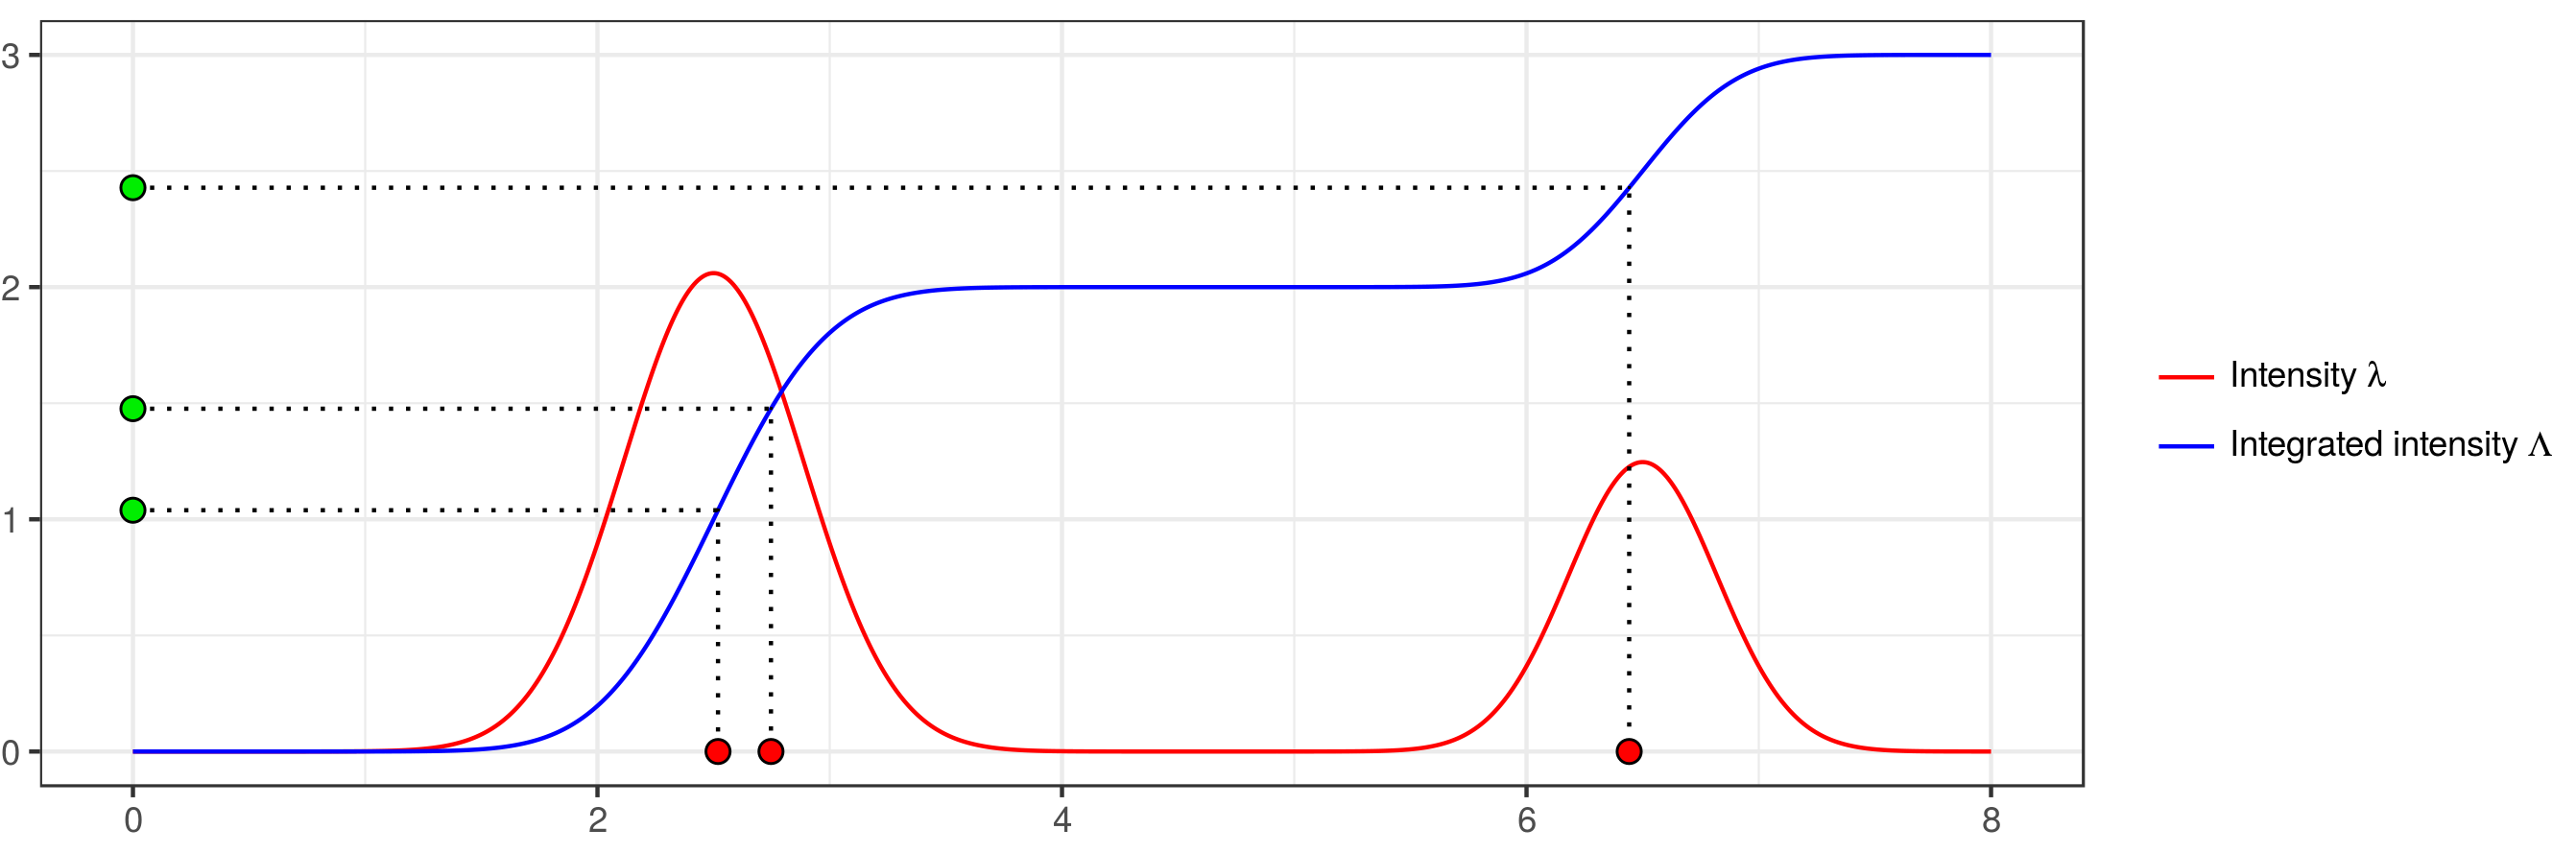
\includegraphics[width=\textwidth]{img/ch2-pp-time-scale}
  \caption{The time scale transformation method for simulating a
  non-homogeneous Poisson process with intensity function $\lambda(t)$.
  We simulate a homogeneous Poisson process (with rate 1) along the y-axis
  and represent the generated samples with the green points.
  After mapping these points along the quantile function of integrated intensity
  $\Lambda$, we obtain
  samples from a non-homogeneous Poisson process with rate $\lambda$, shown
  using the red points on the x-axis.}
  \label{image-pp-time-scale-transformation}
\end{figure}
This algorithm is computationally tractable only for intensity functions
where we can compute line~\ref{alg-line-nhpp-time-scale-intractable-quantile}
quickly; however, most often we do not even have $\Lambda$ in closed form.

\subsubsection{Simulation by thinning}

Suppose $M$ is a non-homogeneous Poisson process with intensity $\lambda(t)$.
Let $\mu(t)$ be a function such that
$\forall t \geq 0 \enskip \lambda(t) \leq \mu(t)$. Then we can think of
$M$ as a thinned out version of a non-homogeneous Poisson process $N$ with
intensity $\mu(t)$ --
an event generated by $N$ at time $t$ is counted (independently of others)
with probability $\frac{\lambda(t)}{\mu(t)}$.
Using \ref{non-hom-pp-characterization} we can derive:
\begin{equation*}
\begin{split}
\pr{\countingProcess{M}{t}{t+h} = 0}
&= \cpr{\countingProcess{M}{t}{t+h} = 0}{\countingProcess{N}{t}{t+h} = 0}
   (1 - \mu(t)h + o(h)) \\
   &\quad+ \cpr{\countingProcess{M}{t}{t+h} = 0}{\countingProcess{N}{t}{t+h} = 1}
   (\mu(t)h + o(h)) \\
   &\quad+ o(h) \\
&= (1 - \mu(t)h + o(h)) + (1 - \frac{\lambda(t)}{\mu(t)} + o(h))
   (\mu(t)h + o(h)) + o(h) \\
   &= 1 - \lambda(t)h + o(h), \\[0.75em]
\pr{\countingProcess{M}{t}{t+h} = 1}
&= \cpr{\countingProcess{M}{t}{t+h} = 1}{\countingProcess{N}{t}{t+h} = 1}
   (\mu(h) + o(h)) + o(h) \\
&= \lambda(t)h + o(h).
\end{split}
\end{equation*}
Also, the independent increments property for $M$ holds (since it does for $N$) and
hence $M$ is a non-homogeneous Poisson process with intensity $\lambda(t)$ as required.
We provide the pseudocode for the above technique in
Algorithm~\ref{alg-non-hom-pp-thinning}.

\begin{algorithm}
\caption{Non-homogeneous Poisson process simulation by thinning}
\label{alg-non-hom-pp-thinning}
\begin{algorithmic}
  \State{$T \gets 0$}
  \Comment{Last event time of a Poisson process $N$ with intensity
           $\mu(t) \geq \lambda(t)$}
  \For{$i = 1, 2, \dots$}
    \State{$\text{counted} \gets \textbf{false}$}
    \While{$\textbf{not } \text{counted}$}
      \State{$T \gets \text{next sample from $N$
        (given by, for example, Algorithm~\ref{alg-non-hom-pp-time-scale})}$}
      \State{$\text{Generate } U \sim \text{Uniform}(0, 1)$}
      \State{$\algorithmicif\ U \leq \frac{\lambda(T)}{\mu(T)}\
              \algorithmicthen\ \text{counted} \gets \textbf{true}$}
    \EndWhile
    \State{$T_{i} \gets T$}
  \EndFor
\end{algorithmic}
\end{algorithm}

\subsubsection{Simulation by the composition method}

The technique to be presented plays a crucial role in the big-data
setting as we will see in the following chapters.
It will allow us to exploit special structual properies of probability distributions
for efficient simulation.

Sometimes the intensity function $\lambda(t)$ can be naturally represented
as a sum of non-negative functions: $\lambda(t) = \sum_{i=1}^{m} \lambda_{i}(t)$.
Denote the associated integrated intensity functions by $\Lambda_{i}(t)$.
Let the main Poisson process be $N$, and denote by $N_{i}$ a Poisson process induced
by the intensity function $\lambda_{i}(t)$. Assume further that processes
$N_{1}, N_{2}, \dots, N_{m}$ are independent.
Then, to simulate the first event time $T$ of Poisson process $N$ we can simulate event times
$T_{i}$ of processes $N_{i}$ for $i \in \{1, 2, \dots, m\}$ and take
the minimum.
To see why this works, let $E_{i}$ be i.i.d. $\text{Exp}(1)$ random variables and
note that:
\begin{align*}
  \pr{T_{1} > t, T_{2} > t, \dots, T_{m} > t}
  &= \prod_{i=1}^{m} \pr{T_{i} > t} && \text{(by independence)} \\
  &= \prod_{i=1}^{m} \pr{E_{i} > \Lambda_{i}(t)} && \text{(by Algorithm~\ref{alg-non-hom-pp-time-scale})} \\
  &= \prod_{i=1}^{m} \exp(-\Lambda_{i}(t)) \\
  &= \exp(-\Lambda(t)) \\
  &= \pr{T > t}.
\end{align*}
Assume that the first event time $t_{1}$ was induced
by the process $N_{k}$.
To simulate the second event time $t_{2}$, we can repreat the same procedure:
simulate the first event times of Poisson processes with intensity
functions \mbox{$\lambda_{i}'(t) \coloneqq \lambda_{i}(t + t_{1})$},
take the minimum and add $t_{1}$ to the result.
Now comes the great part -- instead of resimulating event times for all
processes, we can reuse the results we got before and only simulate the next
event for process $k$.
To see why this is true, note that for $i \neq k$ we have:
\begin{align*}
\cpr{T_{i} > t}{T_{i} > t_{1}}
&= \cpr{E_{i} > \Lambda_{i}(t)}{E_{i} > \Lambda_{i}(t_{0})} \\
&= \pr{E_{i} > \Lambda_{i}(t) - \Lambda_{i}(t_{1})} \\
&= \pr{E_{i} > \Lambda_{i}'(t - t_{1})} \\
&= \pr{\countingProcess{N_{i\,}}{t_{1}}{t} = 0}.
\end{align*}
This concludes the proof of correctness for simulation via the composition method.
See Algorithm~\ref{alg-pp-composition-method} for pseudocode.

We end this section by providing a more intuitive argument as to why
this algorithm is valid.
Note that for the main Poisson process $N$, the probability of exactly one event happening
in $(t, t+h)$ is $\lambda(t) + o(h)$. We can rewrite it as:
$$
\lambda(t) + o(h)
= \left( \sum_{i=1}^{m} \lambda_{i}(t) \right) + o(h)
= \sum_{i=1}^{m} \left( \lambda_{i}(t) + o(h) \right).
$$
Each term in the RHS of the above equation show the contribution of processes $N_{i}$
to the main process $N$.
Hence simulating events from individual components $N_{i}$ and ordering the
event times yield the event times of Poisson process with rate $\lambda(t)$.




\begin{algorithm}
\caption{Non-homogeneous Poisson process simulation by the composition method}
\label{alg-pp-composition-method}
\begin{algorithmic}
  \State{$D \gets \text{Some data structure for efficient storage of event times (e.g. heap)}$}
  \For{$i = 1, 2, \dots, m$}
    \State{$T_{i} \gets \text{The first event time of Poisson process } N_{i}$}
    \State{Insert $(T_{i}, i)$ to $D$ where the elements are ordered by the first parameter.}
  \EndFor
  \For{$i = 1, 2, \dots$}
    \State{$(T, k) \gets \text{An element with the smallest time in $D$}$}
    \State{$T_{k} \gets \text{Simulate the next event time of Poisson process $N_{k}$ }$}
    \State{Insert $(T_{k}, k)$ to $D$}
    \State{$T^{(i)} \gets T$}
    \Comment{Set the $i$-th event time of the main Poisson process.}
  \EndFor
\end{algorithmic}
\end{algorithm}

\section{Markov Processes and their Infinitesimal Generators}

First, we briefly recall how a Markov process is defined.
Let $(X_{t})_{t \geq 0}$ be a stochastic process
taking values in some measurable space $(E, \mathcal{E})$.
Let $\{\mathbb{P}_{x} \mid x \in E \}$
\footnote{
  We also assume that the randomness of our Markov process is carried by
  letting $X_{t} = X_{t}(\omega)$, where $\omega \in \Omega$. Further, we assume
  that $(X_{t})_{t \geq 0}$ is adapted to some filtration $\{\mathcal{F}_{t}\}$
  and $\forall x\nobreak\in\nobreak E \enskip
  (\Omega, \mathcal{F}, \{\mathcal{F}_{t}\}, \mathbb{P}_{x})$
  is a filtered probability space.
}
be a collection of probability measures and further define the \textit{transition function}
\mbox{$P : \mathbb[0, \infty) \times E \times \mathcal{E} \to [0, 1]$} by:
$$P(t, x, \Gamma) = \mathbb{P}_{x}(\{X_{t} \in \Gamma\}).$$
It represents the probability, that our
process, started at position $x \in E$,
is in some set $\Gamma \in \mathcal{E}$ at time $t$.
Finally, we require that
$\forall t,s \geq 0, x \in E, \Gamma \in \mathcal{E}$
$$\mathbb{P}_{x}(\{x_{t+s} \in \Gamma\} \mid \mathcal{F}_{t}) = P(s, x_{t}, \Gamma)
  \enskip \text{(a.s. with respect to $\mathbb{P}_{x}$)}.$$
This condition ensures the \textit{Markov property} -- the evolution of the process
after time $t$ is independent of the past if we know the value of the process
at time $t$. See the classical monograph by
\citet[Chapter 3]{dynkin1965markov} for more details and a rigorous definition
of Markov processes.

One can view the transition function as a family of linear operators
$\{P_{t}\}_{t \geq 0}$ acting on bounded $\mathcal{E}$-measurable functions $f$
by:
$$P_{t}f(x) = \myintNoVariable{E}{}{f(y)P(t, x, dy)}.$$
From the Markov property, we can deduce that $\{P_{t}\}$ forms a (contraction)
semigroup in the following way:
$$\forall t,s \geq 0 \enskip P_{t}P_{s} = P_{t+s}.$$

Sometimes, instead of defining the transition function,
it is easier to define a Markov process in terms of its movement on
an infinitesimal time scale. An \textit{infinitesimal generator} $\mathcal{A}$
of a semigroup $\{P_{t}\}$ is given by:
\begin{equation}
  \label{infinitesimal-generator-definition}
  \mathcal{A}f(x) = \lim_{t \to 0^{+}} \frac{P_{t}f(x) - f(x)}{t}.
\end{equation}
We denote the set of functions for which the above limit is well-defined by
$\mathcal{D}_{\mathcal{A}}$ and call it the \textit{domain} of $\mathcal{A}$.
Intuitively, for small $t$ we expect that
$$P_{t}f(x) \approx f(x) + t\mathcal{A}f(x)$$
should hold.
Under some very
mild assumptions, the infinitesimal generator uniquely determines the
transition function of the associated transition semigroup. See
\cite[Chapters 1 and 2]{dynkin1965markov}
for discussion on infinitesimal
operators of contraction semigroups and relation to the transition functions.

For MCMC applications, we are particularly interested in
\textit{invariant distributions}. A probability measure $\mu$ is invariant,
if a Markov process distributed according to $\mu$ at time $0$,
stays at distribution $\mu$ forever. More formally, a probability measure
$\mu$ on $(E, \mathcal{E})$ is invariant for the Markov process defined above, if:
$$\forall \Gamma \in \mathcal{E} \enskip \forall t \geq 0 \enskip \mu(\Gamma)
  = \myintNoVariable{E}{}{P(t, x, \Gamma)\mu(dx)}.$$
Verifying the above equation is often very hard.
An alternative way to check if $\mu$ is an invariant distribution is available
if we know the infinitesimal generator $\mathcal{A}$ of our process.
Since for invariant measure $\mu$ the distribution of our process does not change
over time and since $\mathcal{A}$ describes the movement of our process,
we expect that on average, our process "does not move" with respect to $\mu$,
if $\mu$ is invariant.
Indeed, it was shown in
\cite[Proposition 34.7] {davis1993markov} that $\mu$ is invariant if and only if:
\begin{equation}
  \label{infinitesimal-generator-invariance}
  \forall f \in \mathcal{D}_{\mathcal{A}} \enskip
  \myintNoVariable{E}{}{\mathcal{A}f(x)\mu(dx)} = 0.
\end{equation}

To help better understand the infinitesimal generators of Markov processes, we
finish this section with a concrete example.
Let $N_{t} \coloneqq N(0, t]$ be a homogeneous Poisson process (following the
notation from Section~\ref{background-material-poisson-processes})
with rate $\lambda > 0$. Recall that the interarrival times follow i.i.d
$\text{Exp}(\lambda)$ distribution. By the momoryless property of the exponential
distribution (it is in fact the only continuous time distribution having such
property), one can deduce that the process starts afresh at every time step
$t > 0$ in the sense that $N_{s}^{t} \coloneqq N_{t + s} - N_{t}$ is again a
Poisson process with rate $\lambda$. So $(N_{t})_{t \geq 0}$ is a Markov process.
What can we say about its infinitesimal generator $\mathcal{A}$? Let $f$ be some
function defined on $\mathbb{N}_{\geq 0}$.
By Equation~\ref{hom-pp-characterization}
we have:
$$P_{h}f(n) = f(n)(1 - \lambda h + o(h)) + f(n+1)(\lambda h + o(h)) + o(h)$$
and hence by Equation~\ref{infinitesimal-generator-definition} we deduce that
\begin{equation}
  \label{pp-infinitesimal-generator}
  \mathcal{A}f(n) = \lambda(f(n+1) - f(n)).
\end{equation}
This expression is not surprising -- on an infinitesimal time scale our function $f$
can only change by $f(n+1) - f(n)$ while the rate $\lambda$ controls how often
such changes can occur.


\section{Piecewise-Deterministic Markov processes}

We will now introduce a class of stochastic processes governed by random jumps at
a sequence of random times $T_{1} < T_{2} < \dots$ and deterministic motion
in-between. Piecewise-deterministic Markov processes (PDMP) were introduced by
\citet{davis1984piecewise} where it was claimed
that this class of stochastic processes is rich enough to include virtually
all non-diffusion models in applied probability.
The material below is not presented in full generality
and mathematical rigour; instead, we attempt to provide an intuitive
understanding to feel comfortable with the following chapters of this project
report.
We refer to the textbook by \citet{davis1993markov}.

\subsection{The definition}
\label{pdmp-definition}

A PDMP is determined by the three \textit{local characteristics}
$(\phi, \lambda, \mathcal{Q})$:

\begin{enumerate}
  \item Let $\phi : \mathbb{R}^{d} \times \mathbb{R} \to \mathbb{R}^{d}$
        be a continuous map differentiable in its second parameter such that
        $\forall t,s \in \mathbb{R} \enskip
        \phi(\cdot, t + s) = \phi(\phi(\cdot, s), t)$.
        We call $\phi$ the \textit{flow function} since the PDMP process evolves
        deterministically according to $\phi$ in-between the jump times.
  \item The \textit{jump rate}
        $\lambda : \mathbb{R}^{d} \to \mathbb{R}_{+}$
        together with the flow determines the jump times $T_{1}, T_{2}, \dots$
        In particular, if the current time is $t$ and the process is at state
        $x \in \mathbb{R}^{d}$, the next jump time $t + T$ is determined by
        the first arrival time $T$ of a non-homogeneous Poisson process
        with intensity function
        $\lambda(\phi(x, \cdot))$. We assume that
        $\forall x \in \mathbb{R}^{d} \enskip \exists \varepsilon > 0$ such that
        $\lambda(\phi(x, \cdot))$ is integrable on $(0, \varepsilon)$.

  \item Finally, the actual jumps at the jump times are governed by the
        \textit{Markov kernel}
        $\mathcal{Q} : \mathbb{R}^{d} \times \mathcal{B}(\mathbb{R}^{d})
         \to [0, 1]$
        (i.e. $\forall x \in \mathbb{R}^{d} \enskip \mathcal{Q}(x, \cdot)$
        is a probability measure
        and $\forall B \in \mathcal{B}(\mathbb{R}^{d}) \enskip
        \mathcal{Q}(\cdot, B)$ is measurable).
        We also require that $\forall x \enskip \mathcal{Q}(x, \{x\}) = 0$.
\end{enumerate}

The great thing about PDMPs is that we know precisely what their infinitesimal
generators are. It was shown in \cite[Section 26]{davis1993markov}, that an
infinitesimal generator $\mathcal{A}$ of a PDMP $(\phi, \lambda, Q)$ is given by:
\begin{equation}
  \label{pdmp-infinitesimal-generator}
  \mathcal{A}f(x) = \dv{}{t}f(\phi(x, t)) \Bigr|_{t = 0} +
    \lambda(x) \myintNoVariable{\mathbb{R}^{d}}{}{}{(f(y) - f(x))\mathcal{Q}(x, dy)},
\end{equation}
where $\langle \cdot,\cdot \rangle$ is the dot product.
The domain $\mathcal{D}_{\mathcal{A}}$ of the generator $\mathcal{A}$
is also shown to be the set of bounded functions $f$ such that
$\forall x \in \mathbb{R}^{d} \enskip f(\phi(x, t))$ is absolutely continuous
as a function of $t$.
As explained in \cite{davis1993markov}, the above expression has an easy
intuitive interpretation.
If $\lambda \equiv 0$, we end up with the first term only, which describes
the deterministic motion of our process. On the other hand, if there is no flow
(i.e. $\forall t,x \enskip \phi(x, t) = x$), then we end up with a generator of
a Markov jump process (see how this relates to Equation~\ref{pp-infinitesimal-generator}).

\subsection{A toy example}
\label{pdmp-toy-example-section}

Suppose we want to model a particle moving along straing lines and changing
direction at random in a two dimensional space. Further, assume that we want to
make it hard for the particle to go too far away from the origin (where the difficulty
increases with the distance from the origin).
We can model such process as a PDMP over the space
$Z = \mathbb{R}^{4} = \mathbb{R}^{2} \times \mathbb{R}^{2} = (X, V)$,
as follows:
\begin{enumerate}
  \item Since we want the particle to move in straight lines, we can, for example,
    let $\phi(z, t) = \phi((x,v), t) = (x + vt, v)$. That is, we change the particle's
    position $x$ based on velocity $v$. The velocity does not change during the
    deterministic motion.
  \item Now we want to make it hard for the particle to go far away from the origin.
    We can achieve that by letting the jump-rate function $\lambda$ be defined as
    \mbox{$z = (x, v) \mapsto \max\{0, \left\langle x, v \right\rangle\}$}.
    We take the inner product, since we want to take the particle's movement
    direction into account. We also take the maximum function, since the jump rate
    must be non-negative. Note that in such a scenario,
    the particle can move freely directly towards the origin. However, as the
    distance from the origin increases, the jump rate also increases, so that the
    particle is more likely to change direction and go back.
  \item At jump times, we leave the particle location unchanged, but sample a new
    velocity uniformly from,
    $S^{1} \coloneqq \{(v_{1}, v_{2}) \in \mathbb{R}^{2} \mid v_{1}^{2} + v_{2}^2 = 1 \}$.
\end{enumerate}

See Figure~\ref{image-pdmp-simple} for a sample simulation of this process.
The Bouncy Particle Sampler is a very similar algorithm. By carefully choosing
the jump rate function and the transition kernel, we will be able to guide our
particle, so that the resulting invariant distribution is the one we want to sample from.
We will see in Chapter~\ref{chapter-bouncy-particle-sampler} how the BPS algorithm
was derived and why it works.

\begin{figure}
  \begin{subfigure}{.5\textwidth}
    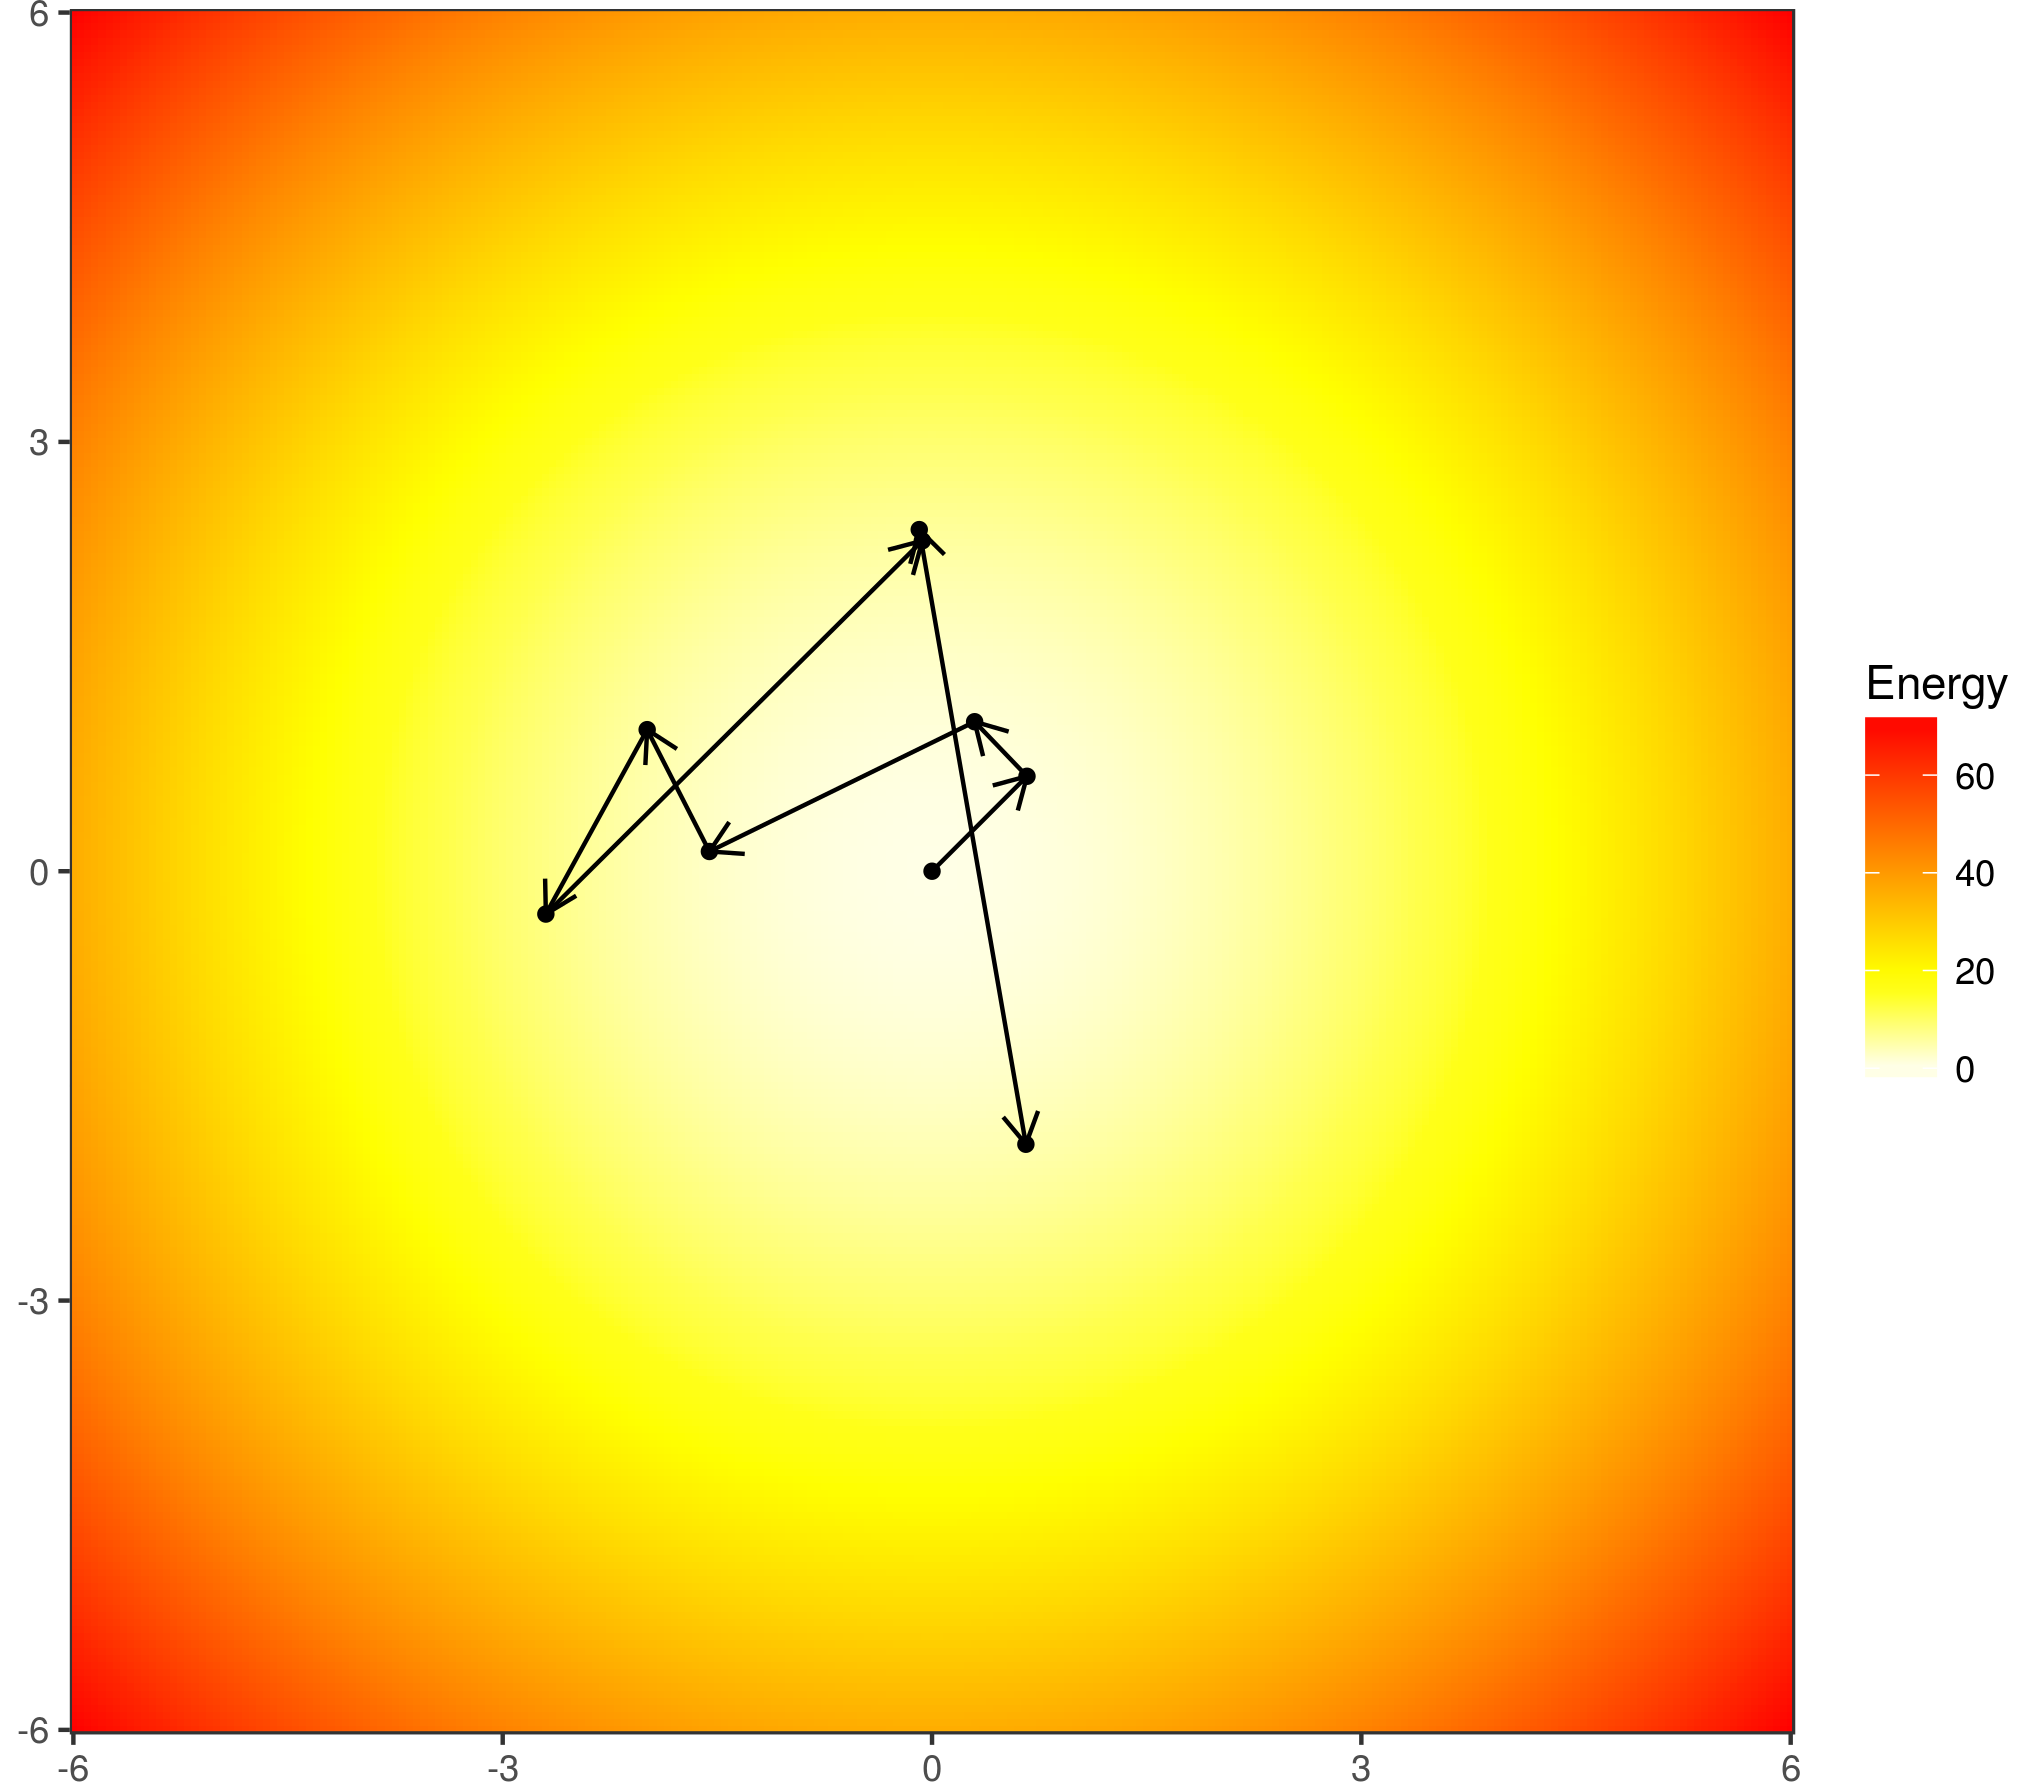
\includegraphics[width=\textwidth]{img/ch2-pdmp-simple}
    \caption{}
    \label{image-pdmp-simple-short}
  \end{subfigure}
  \begin{subfigure}{.5\textwidth}
    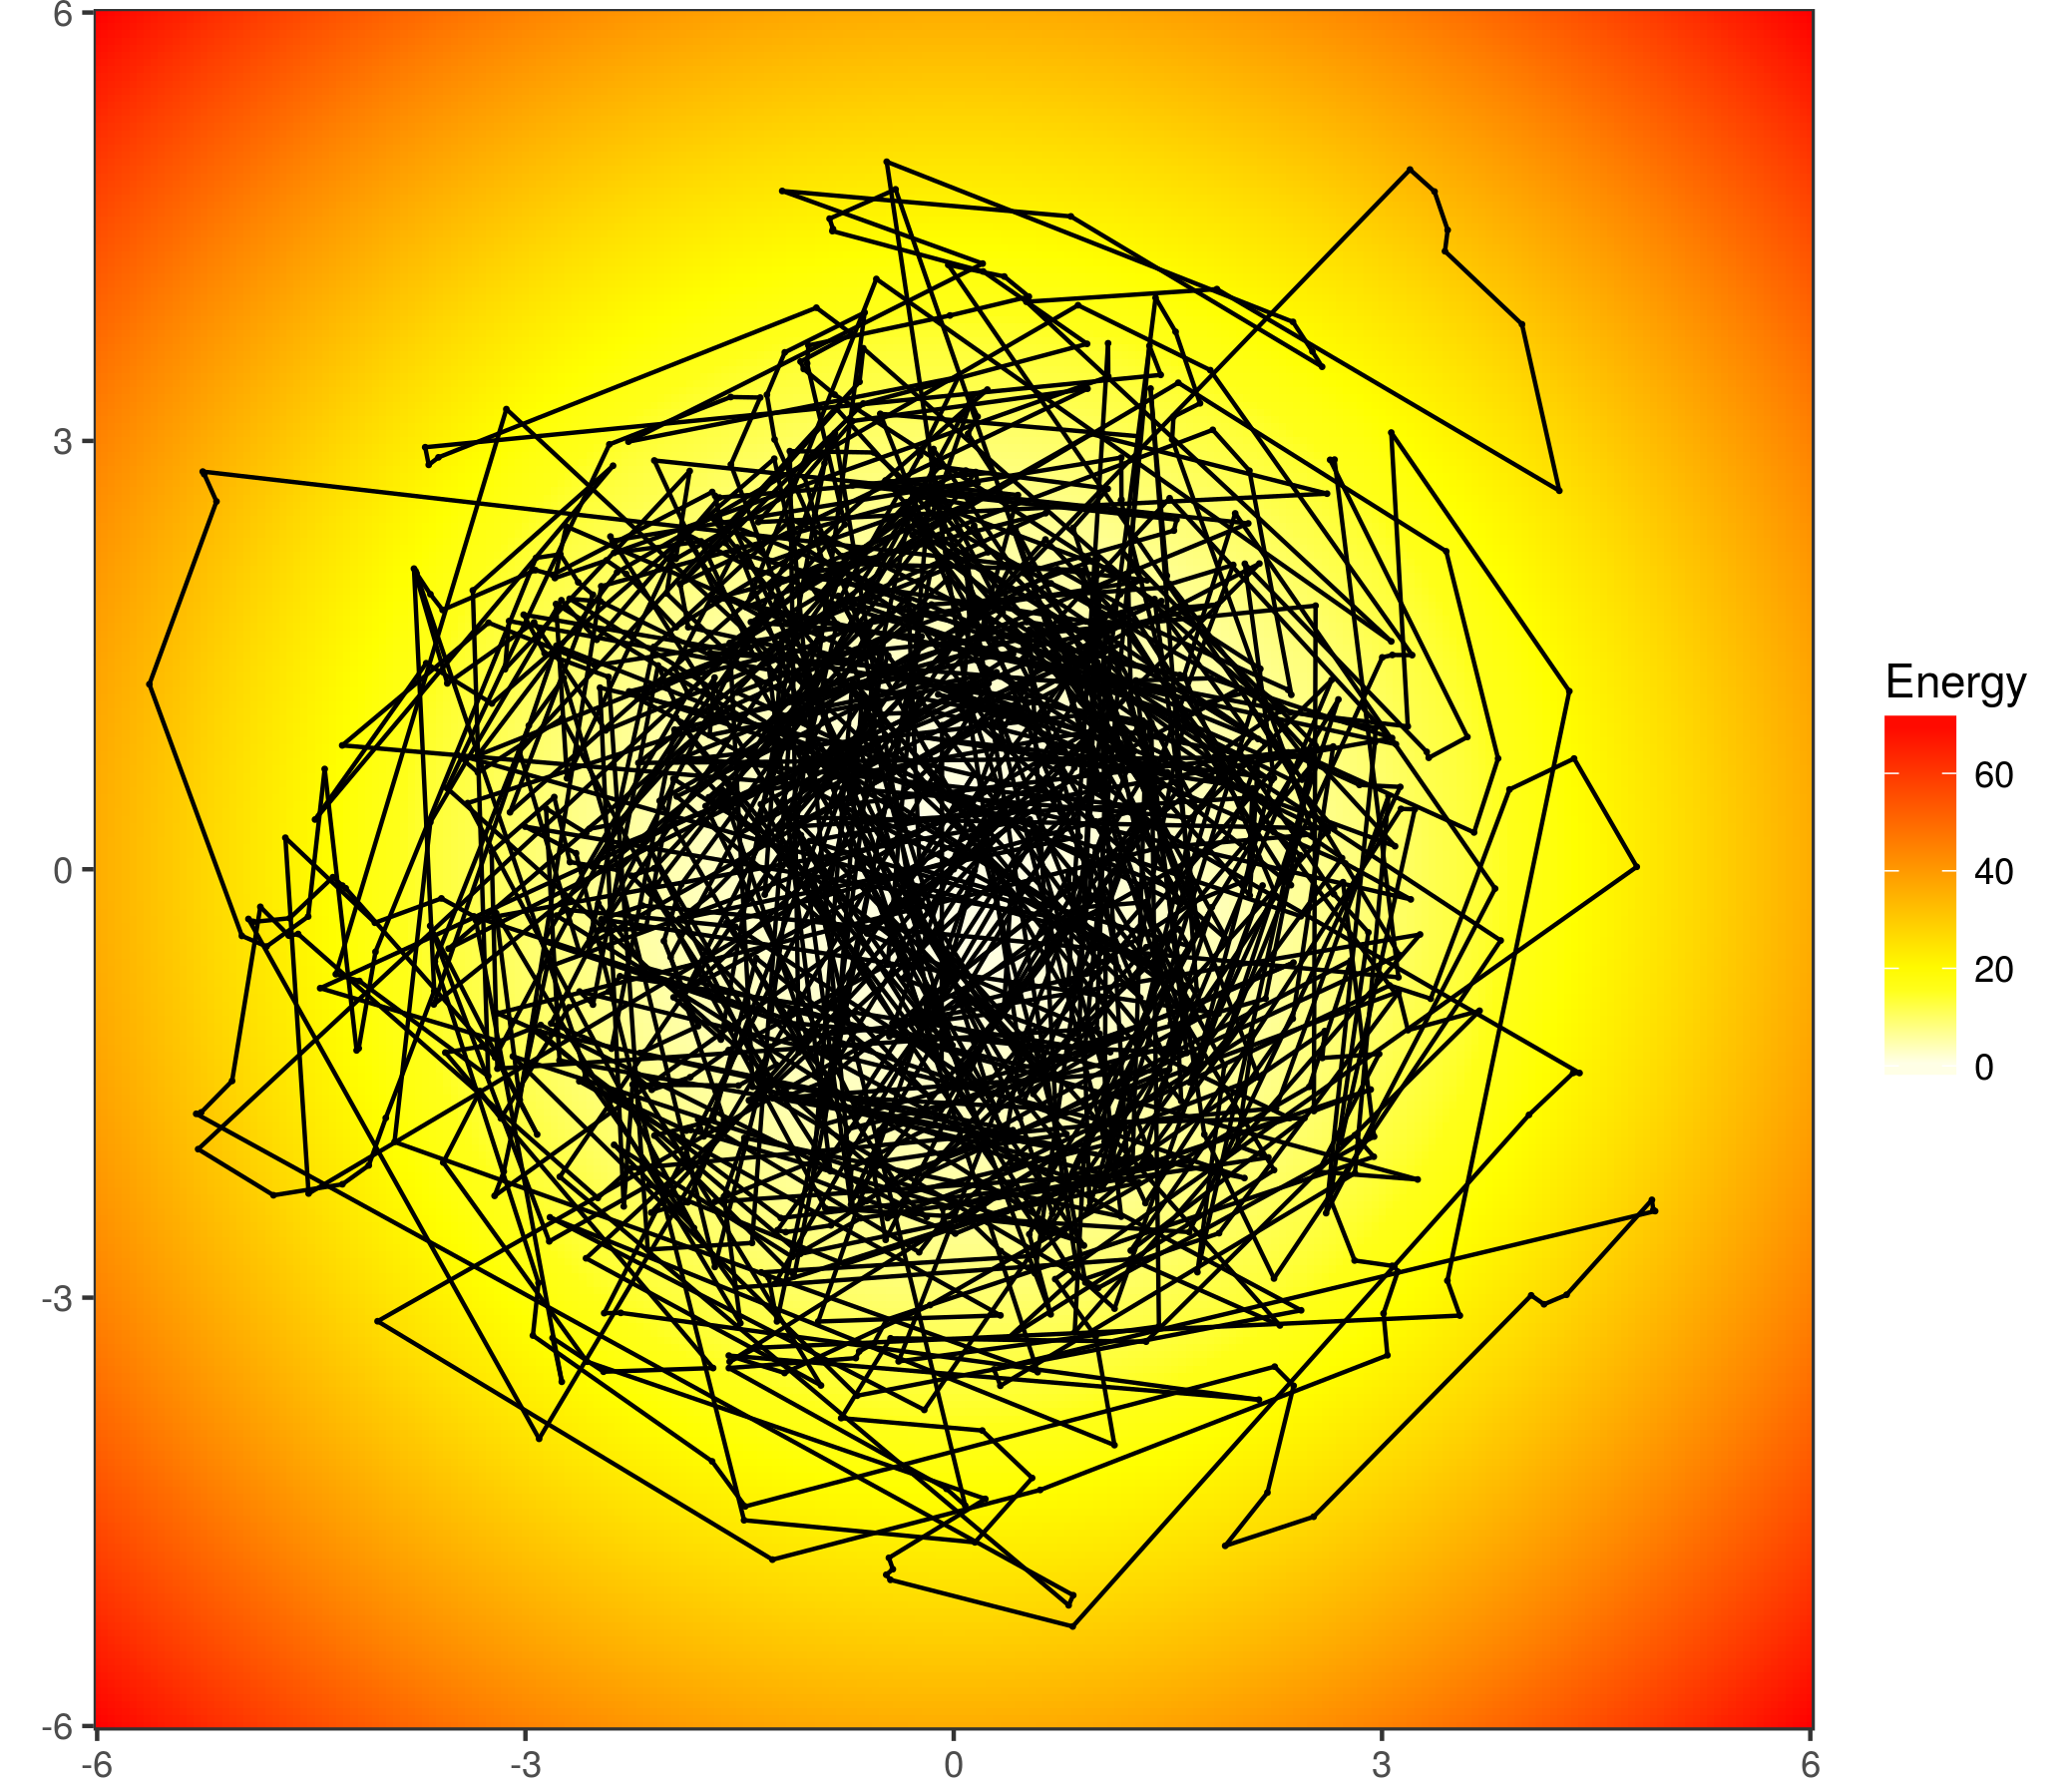
\includegraphics[width=\textwidth]{img/ch2-pdmp-simple-gaussian}
    \caption{}
    \label{image-pdmp-simple-gaussian}
  \end{subfigure}
  \caption{The toy example considered in Section~\ref{pdmp-toy-example-section}.
    Figure~\subref{image-pdmp-simple-short} shows the first $7$ simulated events.
    We can see how the process evolved after $1000$ events in
    Figure~\subref{image-pdmp-simple-gaussian}.}
  \label{image-pdmp-simple}
\end{figure}



\end{document}

